\documentclass[UTF8, xcolor=table]{beamer}
%\usepackage{fontspec}
%\setsansfont{宋体}
\usepackage[BoldFont,SlantFont]{xeCJK}
\setCJKmainfont[BoldFont={Adobe Heiti Std},ItalicFont={Adobe Kaiti Std}]{SimSun}

\usepackage{latexsym,amssymb,amsmath,amsbsy,amsopn,amstext,xcolor,multicol}
\usepackage{graphicx,wrapfig,fancybox}
\usepackage{pgf,pgfarrows,pgfnodes,pgfautomata,pgfheaps,pgfshade}
\usepackage{thubeamer}
%\usepackage[backend=bibtex,style=IEEE,sorting=none]{biblatex} % [参考文献格式](https://www.sharelatex.com/blog/2013/07/31/getting-started-with-biblatex.html)
\usepackage[backend=bibtex,sorting=none]{biblatex} % [参考文献格式](https://www.sharelatex.com/blog/2013/07/31/getting-started-with-biblatex.html) %mac IEEE not found
\usepackage{array}
\usepackage{bm}
\usepackage{caption}
\usepackage[caption=false,font=scriptsize]{subfig}
\usepackage{multirow}
\usepackage{booktabs}
\usepackage{tikz}
\usepackage{tikzscale}
\usepackage{animate}
%\usepackage{times} %与上面的冲突,加上这个 粗体斜体就失效
%\usepackage{mathptmx}


\defbibheading{bibliography}[\bibname]{} %avoid printbibliography 自动生成目录
\addbibresource{ref/papers-bib-in-google.bib}
\addbibresource{ref/chinese-ref.bib}
%\setbeamertemplate{bibliography item}{\insertbiblabel} %将列表中默认的丑陋的icon 改成数字,或者下面这个也行
\setbeamertemplate{bibliography item}[text] % [ref](http://tex.stackexchange.com/questions/68080/beamer-bibliography-icon)
%\setbeamertemplate{footline}[frame number]{}

%\setframeofframes{of}

\usepackage{boxedminipage} %for: bvh border
\def\fourgraphicswidth{0.35} %0.3\textwidth

\usepackage{algorithm} %%format of the algorithm
\usepackage{algpseudocode}
\floatname{algorithm}{算法}
\renewcommand{\algorithmicrequire}{\textbf{输入:}} %%Use Input in the format of Algorithm
\renewcommand{\algorithmicensure}{\textbf{输出:}} %%UseOutput in the format of Algorithm
%\algrenewcommand{\algorithmiccomment}[1]{\hskip3em $\rightarrow$ #1}
\algrenewcommand{\algorithmiccomment}[1]{ $//$ #1}

\usepackage{listings}
\renewcommand\lstlistingname{代码}
\renewcommand\lstlistlistingname{代码}

\lstset{framexleftmargin=1.4em,
        xleftmargin=1.8em,
        basicstyle=\ttfamily\small,
        %frame=shadowbox, numberstyle=\tiny, breaklines=true,
        frame=single,
        numberstyle=\tiny, breaklines=true,
        keywordstyle=\color{blue!70}\bfseries,
        %commentstyle=\color{red!50!green!50!blue!50},
        rulesepcolor=\color{red!20!green!20!blue!20},
        numbers=none,fontadjust=true}
\lstdefinelanguage{shader}{morekeywords={uniform, layout, uniform, vec2, vec3, vec4, in, out, gl_Position, dot, flat, int ,float, gl_VertexID, xyz, w, x, y, z, location, version, sampler2DRect, bgr, gl_FragData, texture2DRect, gl_TexCoord,for,xy},morecomment=[l]{//}}

%\setbeameroption{show notes} %un-comment to see the notes

%\usepackage{pgfpages}
%\renewcommand\pgfsetupphysicalpagesizes{%
%    \pdfpagewidth\pgfphysicalwidth\pdfpageheight\pgfphysicalheight%
%}
%\setbeameroption{show notes on second screen}

\begin{document}

\setbeamerfont{footnote}{size=\tiny}
\setbeamerfont{caption}{size=\scriptsize}
\setbeamertemplate{caption}[numbered]
\setbeamerfont{subsection in toc}{size=\footnotesize}
\renewcommand*{\bibfont}{\footnotesize}

\graphicspath{{figures/}}

\title{凸包围多面体生成算法及应用}
%\author{唐磊}
\author[唐磊]{(申请清华大学工学硕士学位论文答辩报告)\vskip 20pt学~~~~~~生:唐~~~~~磊~~~~~~~~\vskip 5pt 指导教师:雍~俊~海~教授}
\institute[清华大学~软件学院~CG~\&~CAD~研究所]{\small \vskip 38pt计算机辅助设计图形学与可视化研究所}
%\date{2015-06-07}
\date{\small \vskip -17pt二〇一五年六月}
%\date{\today}



\frame{
\vspace{-15mm}
\titlepage
\vspace{-43mm}
\begin{figure}[htbp]
  \begin{center}
	
\includegraphics[width=0.16\linewidth]{Tsinghua_University_Logo.eps}
  \end{center}
\end{figure}
%\beign{picture}(1,1)
%\put(6,8){
\includegraphics[width=0.15\linewidth]{Tsinghua_University_Logo.eps}}
%\end{picture}
}

  \section*{目录}
  \frame {
    \frametitle{\secname}
   % \begin{multicols}{2}
    \tableofcontents[sections={<1-5>}]
  %\end{multicols}
    \note{
      我将按照下面如下的次序来介绍本人的工作,首先是课题背景和相关工作,然后介绍凸包围体生成算法和基于凸包围体的碰撞检测算法,最后进行总结。
    }
  }

  \AtBeginSubsection[] {
  \frame<handout:0> {
  \frametitle{目录}
  \tableofcontents[current,currentsubsection,sections={<1-5>}]
    }
    \addtocounter{framenumber}{-1}  %目录页不计算页码
  }

  \section{背景}
  \frame
  {
    \frametitle{\secname~ }
    \begin{block}{凸包围体技术}
      在计算机图形学领域里的各种算法中发挥着重要作用,
      如优化渲染和建模过程,加速求交、碰撞检测等算法。
    \end{block}
    \begin{block}{碰撞检测问题}
   计算机图形学、虚拟现实等领域中的研究热点,
   是计算机模拟真实环境中不可或缺的技术,
   在物理仿真及游戏领域里应用十分广泛。
    \end{block}
    \note{
      凸包围体技术在计算机图形学领域里的各种算法中发挥着重要作用,如优化渲染和建模过程,加速求交、碰撞检测等算法。
      主要是用在原始模型之间的相关计算(遮挡测试、相交测试等)之前进行预处理判断和剪枝,以求交算法为例,如果两个模型相交,则对应的凸包围体一定相交,
      若凸包围体不相交则其对应的原始模型一定不相交。而一般来讲,判断凸包围体是否相交比判断原始模型相交更简单,因此可以提升效率。
      
      碰撞检测问题是计算机图形学、虚拟现实等领域中的研究热点,是计算机模拟真实环境中不可或缺的技术,在物理仿真及游戏领域里应用十分广泛。
      例如在游戏中,碰撞检测技术增强了游戏的真实性,游戏中的角色行走不可穿墙、角色中弹而亡等等都离不开碰撞检测技术。
    }
  }

  \subsection{凸包围体}
  \frame{
  \frametitle{凸包围体的种类}
  \begin{figure}
  \hspace{-2.0em}
    \begin{minipage}{1.06\textwidth}
    \subfloat[\scriptsize AABB]
        {
           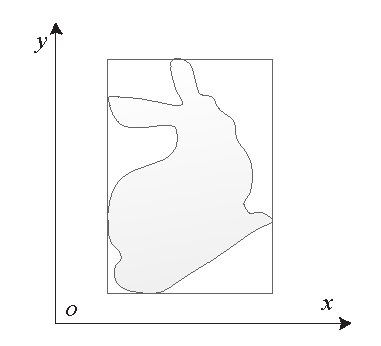
\includegraphics[width=0.2\textwidth]{figures/bunny-2d-AABB.eps}
        }
        \subfloat[\scriptsize OBB]
        {
            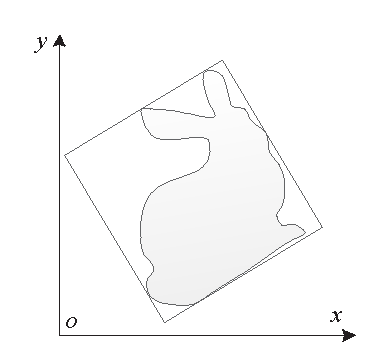
\includegraphics[width=0.2\textwidth]{figures/bunny-2d-OBB.eps}
        }
       \subfloat[\scriptsize Sphere]
        {
           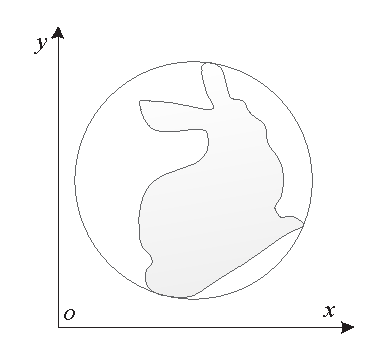
\includegraphics[width=0.2\textwidth]{figures/bunny-2d-Sphere.eps}
        }%\linebreak
        \subfloat[\scriptsize $k$-DOP]
        {
           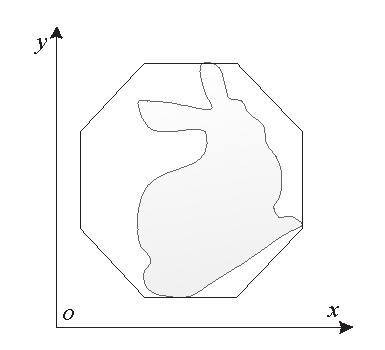
\includegraphics[width=0.2\textwidth]{figures/bunny-2d-8DOP.eps}
        }
        \subfloat[\scriptsize 凸包]
        {
           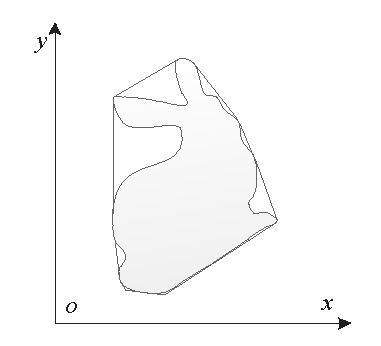
\includegraphics[width=0.2\textwidth]{figures/bunny-2d-Convexhull.eps}
        }
        \end{minipage}
        \caption{不同种类的包围体}
        \label{chart:exps:tightness}
        \end{figure}
        \vspace{-1em}
      其他:Tribox、Swept-sphere、 Sphere-shell、Zonotopes、圆柱形、圆锥、椭球形等等。
      
      \note{
        上面这几个就是最常见的凸包围体。最常见的沿坐标轴方向的AABB包围盒,带方向的包围盒OBB,包围球,k面的凸包围体(k-DOP),和凸包,还有一些比较特定领域用的圆柱、圆锥形、椭球形等等。
        其中k-DOP是采用k/2对固定方向的半空间相交构成的凸包围体,是综合比较较好的包围体,因为可以通过k来调节包围体的简单性和紧致性来满足不同应用的需求。
      }
  }

      \frame{
   \frametitle{本文目标}
     \footnotesize
     \textbf{$k$-DOP}\footfullcite{klosowski1998efficient}的局限性:方向\textbf{固定}且为\textbf{有限的偶数},不同模型其截面方向一致, \textbf{不够紧致};\\ 
     而凸包很(最)紧致,但面片数量太多,构造复杂度$O(n\log n)$。
    \begin{block}{本文凸包围体的目标}
      \hspace{-2.0em}   \begin{minipage}{\textwidth}
    \begin{description}
      \item[紧致:] 能够自适应模型,根据模型形状特点有不同的方向;
      \item[快速:] 生成凸包围体的速度要快,利用~GPU~加速;
      \item[灵活:] 通过参数~$k$~调节凸包围体的简单性和紧致程度。
    \end{description}
  \end{minipage}
    \end{block}

       \note{
         描述PPT。
本文提出的 k-CBP 与 k-DOP 不同之处在于:
(1) k-DOP 中 k 值通常仅局限于少数几个,例如 k = 6,8,14,18,20,26 等,后面那篇文
献最大支持 k = 46),且 k-DOP 中方向是成对平行的,k 值是偶数,而 k-CBP 中
的 k 理论上可以是任意的,奇偶都可以;
(2) k-DOP 中的凸多面体方向是固定的即 k 值确定之后,不管输入模型的点集
分布如何, k-DOP 的方向始终保持一致,本文则提出了一种能够自适应模型的算
法使得构造的凸包围多面体足够紧致;
(3) k-CBP 中 k 取值灵活,必须找出一种算法生成 k 个法向,比只有少数几个可直接通过枚举方向的 k-DOP 取值更复杂。
通过更加紧致的 k-CBP 去近似原始模型,能够达到更好的精度,且输入 k 值
可以自由控制,为其能够用于碰撞检测等应用提供足够大的灵活性。
       }
  }

  \subsection{碰撞检测算法}
   \frame{
   \frametitle{\subsecname~ }
    
   \begin{block}{碰撞检测算法}
     许多应用的基础,例如在~3D~游戏,物理仿真,机器人,虚拟现实等领域中\footfullcite{ericson2005real}。
   \end{block}

   \begin{block}{分类}
     \begin{description}
       \item[加速结构:] SPT(如四叉树、KD~树等)~v.s~\textbf{BVH}(OBB树、$k$-DOP树等)
       \item[表现形式:] \textbf{刚体}~v.s~可变形,凸体~v.s~凹体,CSG~v.s~参数曲面~v.s~\textbf{多边形网格}
       \item[碰撞环境:] \textbf{成对}~v.s~\textbf{多体},\textbf{静止}~v.s~\textbf{运动},\textbf{离散}~v.s~连续
     \end{description}
   \end{block}
   
   \note{
    (介绍PPT后),本文后面的实验就是基于BVH的,不可变形的三角网格。//现在研究较多的是连续的可变形的碰撞检测布料模拟头发模拟等。
   }
  }

  \frame{
    \frametitle{基于~BVH~的碰撞检测算法}
    \begin{columns}[onlytextwidth]
      \begin{column}{0.35\textwidth}
        \vspace{-1.5em}
        \begin{figure}[htbp]
            \begin{center}
            \begin{boxedminipage}{1\textwidth}
            \subfloat{\label{lbl:bvh-bunny-center-0.png}}
              {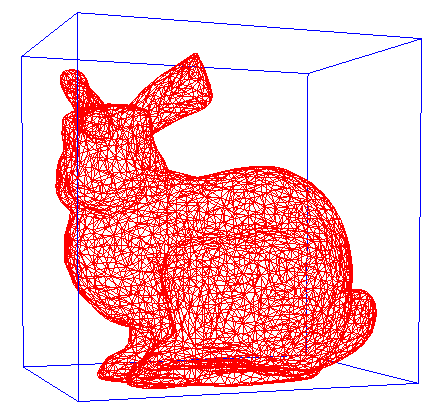
\includegraphics[height=1.4cm]{bvh-bunny-center-0.png}}
            \subfloat{\label{lbl:bvh-bunny-center-1.png}}
              {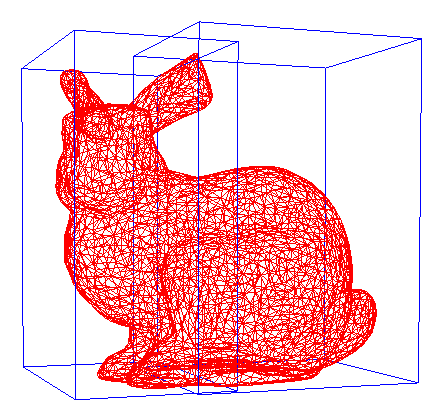
\includegraphics[height=1.4cm]{bvh-bunny-center-1.png}}
            \\
            \subfloat{\label{lbl:bvh-bunny-center-2.png}}
              {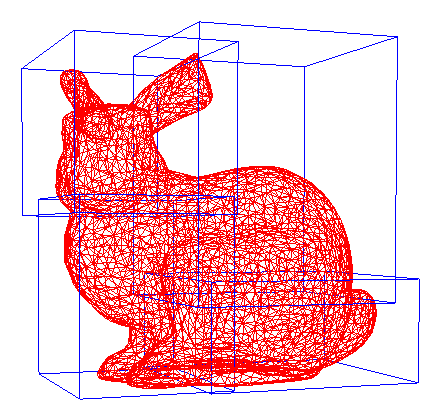
\includegraphics[height=1.4cm]{bvh-bunny-center-2.png}}
            \subfloat{\label{lbl:bvh-bunny-center-3.png}}
              {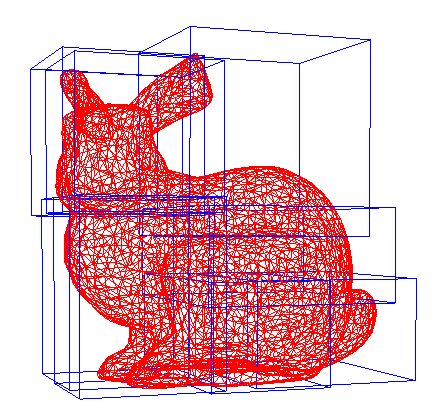
\includegraphics[height=1.4cm]{bvh-bunny-center-3.png}}
            \\\hspace{0.5cm}
            \subfloat{\label{lbl:bvh-bunny-center-4.png}}
              {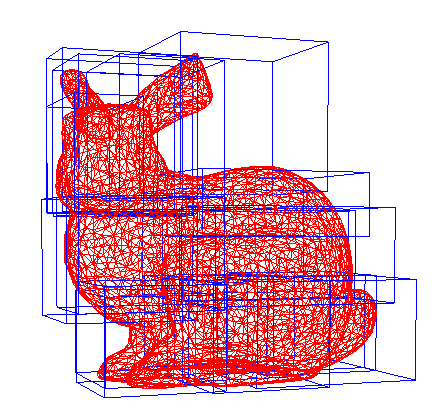
\includegraphics[height=1.5cm]{bvh-bunny-center-4.png}}
            \subfloat{\label{lbl:bvh-bunny-center-5.png}}
              {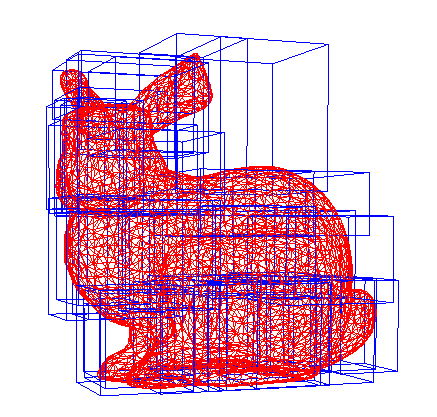
\includegraphics[height=1.5cm]{bvh-bunny-center-5.png}}
            \\
            \subfloat{\label{lbl:bvh-bunny-center-6.png}}
              {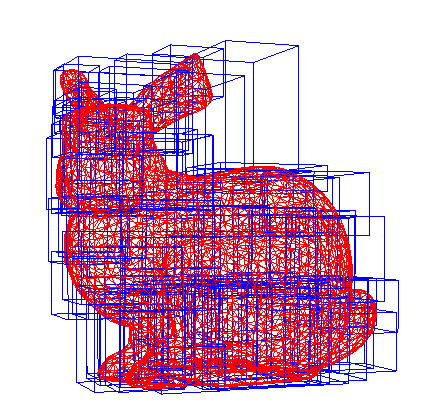
\includegraphics[height=1.5cm]{bvh-bunny-center-6.png}}
            \subfloat{\label{lbl:bvh-bunny-center-7.png}}
              {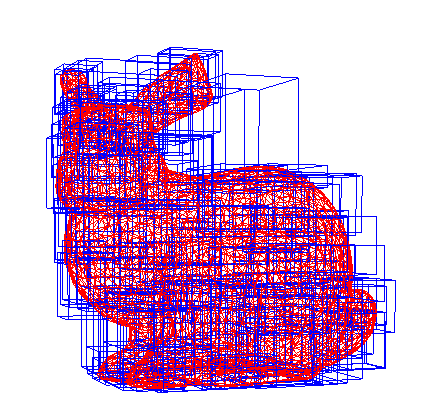
\includegraphics[height=1.5cm]{bvh-bunny-center-7.png}}
            \end{boxedminipage}
            \vspace{-0.5em}
          \caption{八层~BVH~示例}
          \label{lbl:bvh-example}
          \end{center}
          \end{figure}
      \end{column}
      \hspace{0.5em}
      \begin{column}{1.2\textwidth}
      \vspace{0.2em}
         \scalebox{0.5}{
              \begin{minipage}{1.0\textwidth}
      \vspace{-2em}
           \begin{algorithm}[H]
              \caption{自顶向下层次遍历~BVH~}
              \label{alg:traverse-bvh-tree}
              \begin{algorithmic}[1]
              \Require
              两个~BVH~树的根节点~$node_1$,$node_2$
              \Ensure
              模型是否相交
              \Function {TraverseBVHTree}{$node_1, node_2$}
                \If{$node_1.bv \cap node_2.bv = \emptyset$}
                  \State \Return{\textbf{False}}
                  \Comment{包围体重合测试, 包围体不相交直接返回}
                \Else
                    \If {$node_1.children = \emptyset$}
                         \If {$node_2.children = \emptyset$}
                         \State \Comment{最底层叶子节点原生几何相交测试}
                         \State \Return {\Call{CheckIntersection}{$node_1.primitives, node_2.primitives$}}
                         \Else
                            \ForAll {$child \in node_2.children$}
                            \State \Call{TraverseBVHTree}{$node_1, child$} \Comment{递归调用}
                            \EndFor
                         \EndIf
                    \Else
                         \ForAll {$child \in node_1.children$}
                         \State \Call{TraverseBVHTree}{$child, node_2$}  \Comment{递归调用}
                         \EndFor
                    \EndIf
                \EndIf
              \EndFunction
              \end{algorithmic}
              \end{algorithm}
              \end{minipage}
            }
      \\
      \scriptsize \hspace{1em}代价函数: $T_{cost} = n_v * C_v + n_p * C_p + (n_u * C_u)$(运动)
      \end{column}
    \end{columns}
    \note{
      基于包围体树的碰撞检测算法, 一般首先都会初始化环境然后构建层次结构的包围体树,碰撞检测时从顶层开始逐渐往下层遍历,到最底层叶子节点后开始三角网格模型相交测试,
      当发现三角网格相交后立即终止遍历,确定模型发生碰撞。
      评价碰撞检测算法的指标一般用上面这个公式来衡量,其中nv和 np分别表示参与包围体节点相交测试的数量和参与原始几何相交测试的数量,Cv和 Cp则表示相应的平均测试耗费的代价。
      当在运动场景时还需要加上nu和 Cn就是模型旋转或者运动后包围体更新的数量和更新的代价。
      本文算法就是尽早发现包围体不相交的情况,减少np和cp的数量。
    }
}

  
    \section{总结与展望}
    %添加一个目录
    \frame{
     \frametitle{目录}
     \tableofcontents[current,currentsection,sections={<1-5>}]
     \addtocounter{framenumber}{-1}  %目录页不计算页码
    }

    \frame{
      \frametitle{\secname}
      \vspace{-0.5em}
      \begin{block}{总结}
        \footnotesize
        \begin{enumerate}[(1)]
          \item 提出了一种构造紧致凸包围多面体--$k$-CBP~的算法;
          \item 构造~$k$-CBP~速度上比现有算法快~3$\sim$8~倍;
          \item 构造的~$k$-CBP~紧致程度比现有的$k$-DOP紧致10\% $\sim$ 40\%;
          \item 提出了一种基于~$k$-CBP~的碰撞检测算法,该算法较$k$-DOP树算法初始化时间快8倍以上,静止场景快0.8 $\sim$ 3.2 倍,运动场景快0.8 $\sim$ 5.6 倍。
        \end{enumerate}
      \end{block}
      \vspace{-0.5em}
      \begin{block}{展望}
        \footnotesize
      \begin{enumerate}[(1)]
          \item 碰撞检测算法如何摆脱对AABB树的依赖;应用于近似碰撞检测算法;应用于可变形的模型连续碰撞检测,如何快速更新~$k$-CBP~;
          \item 如何将~$k$-CBP~应用于如机器人抓取、路径规划等其他应用领域中。
        \end{enumerate}
      \end{block}
      
      \note{
        总结一下~\ldots PPT
      }
    }

    \section{主要参考文献}
    \frame[t,allowframebreaks]{
      \frametitle{\secname}
    \printbibliography
    }
    
    \section{感谢}
    \frame{
      \frametitle{\secname}
      \begin{block}{致谢}
        \begin{enumerate}[(1)]
          \item 导师雍俊海老师的精心指导;
          \item 施侃乐老师帮助;
          \item 研究所各个项目的历练;
          \item 王斌老师、陈莉老师的评审及意见,答辩委员会老师聆听和指导。
        \end{enumerate}
      \end{block}
    }
    \frame{
      \frametitle{Q \& A}
      \begin{block}{Questions?}
       ~\\ ~\\
       \center{\Large{Thank you!}}
       \\ ~\\ ~\\ ~\\ ~\\ 
      \end{block}
    }



\end{document}

